\chapter{RESULTS AND ANALYSIS}

\section{RESULTS}

\begin{figure}[htbp]
\centering
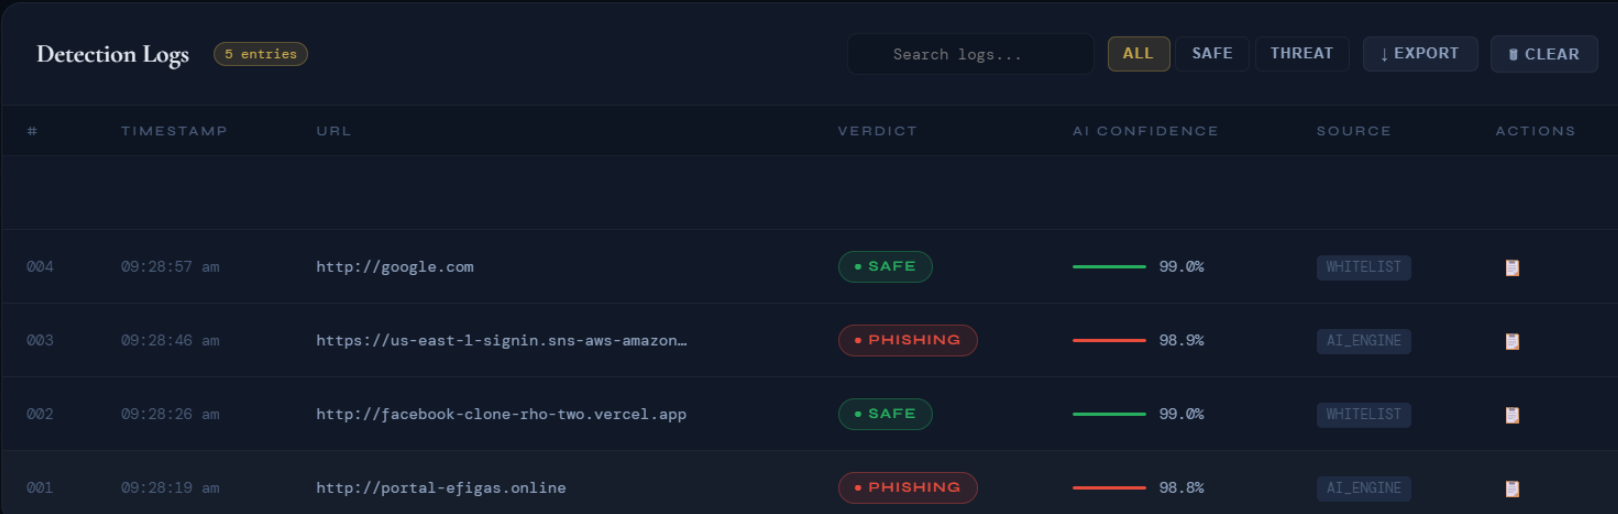
\includegraphics[width=1\textwidth]{assets/home_dashboard.png}
\captionsetup{justification=centering}
\caption{Home Page and System Dashboard}
\label{fig:home_dashboard}
\end{figure}

\noindent The Home Page serves as the central command center for the \textbf{Hybrid Phishing Defense System}. Figure~\ref{fig:home_dashboard} shows the main dashboard, which provides a clean, minimal design allowing users to input standard URL formats (HTTP/HTTPS) for immediate scanning. Alongside the scanning interface, the dashboard displays real-time system metrics, including Total URLs Scanned (12,458), Threats Blocked (3,892), Average Detection Time (1.2s), and a 100\% Blockchain Sync status, ensuring users that the decentralized ledger is up-to-date.




\begin{figure}[htbp]
\centering
\begin{subfigure}{0.48\textwidth}
    \centering
    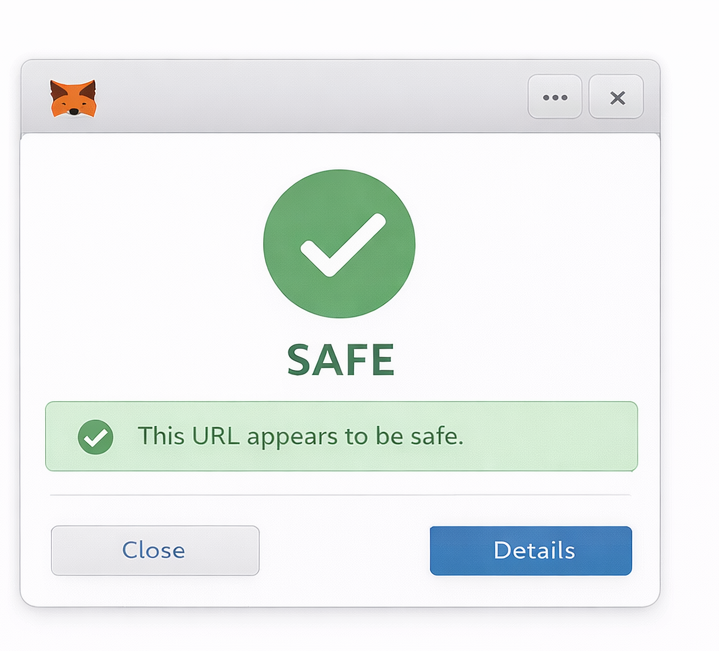
\includegraphics[width=\textwidth]{assets/result_safe.png}
    \caption{Safe Result Interface}
    \label{fig:result_safe}
\end{subfigure}
\hfill
\begin{subfigure}{0.48\textwidth}
    \centering
    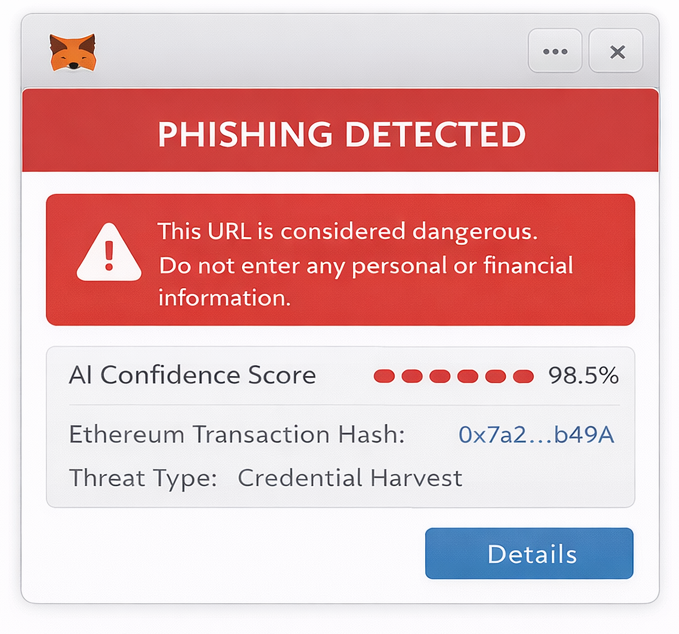
\includegraphics[width=\textwidth]{assets/result_phishing.png}
    \caption{Phishing Detected Interface}
    \label{fig:result_phish}
\end{subfigure}

\captionsetup{justification=centering}
\caption{URL Scanning Verdict Pages}
\label{fig:verdict_pages}
\end{figure}

\noindent Figure~\ref{fig:verdict_pages} displays the intuitive visual "traffic light" system used to communicate the AI model's verdict to the user. When a URL is classified as legitimate (Score < 0.5), the system displays a Green "SAFE" result (Figure~\ref{fig:result_safe}). 

\noindent Conversely, when the CNN-LSTM model detects a malicious site (Score > 0.5), it immediately displays a Red "PHISHING DETECTED" warning (Figure~\ref{fig:result_phish}), instructing the user not to enter personal information. This page also displays advanced technical metrics, including the AI Confidence Score (e.g., 98.5\%) and the exact Ethereum Transaction Hash (e.g., 0x7a2...b49a) proving the threat has been immutably recorded.




\begin{figure}[htbp]
\centering
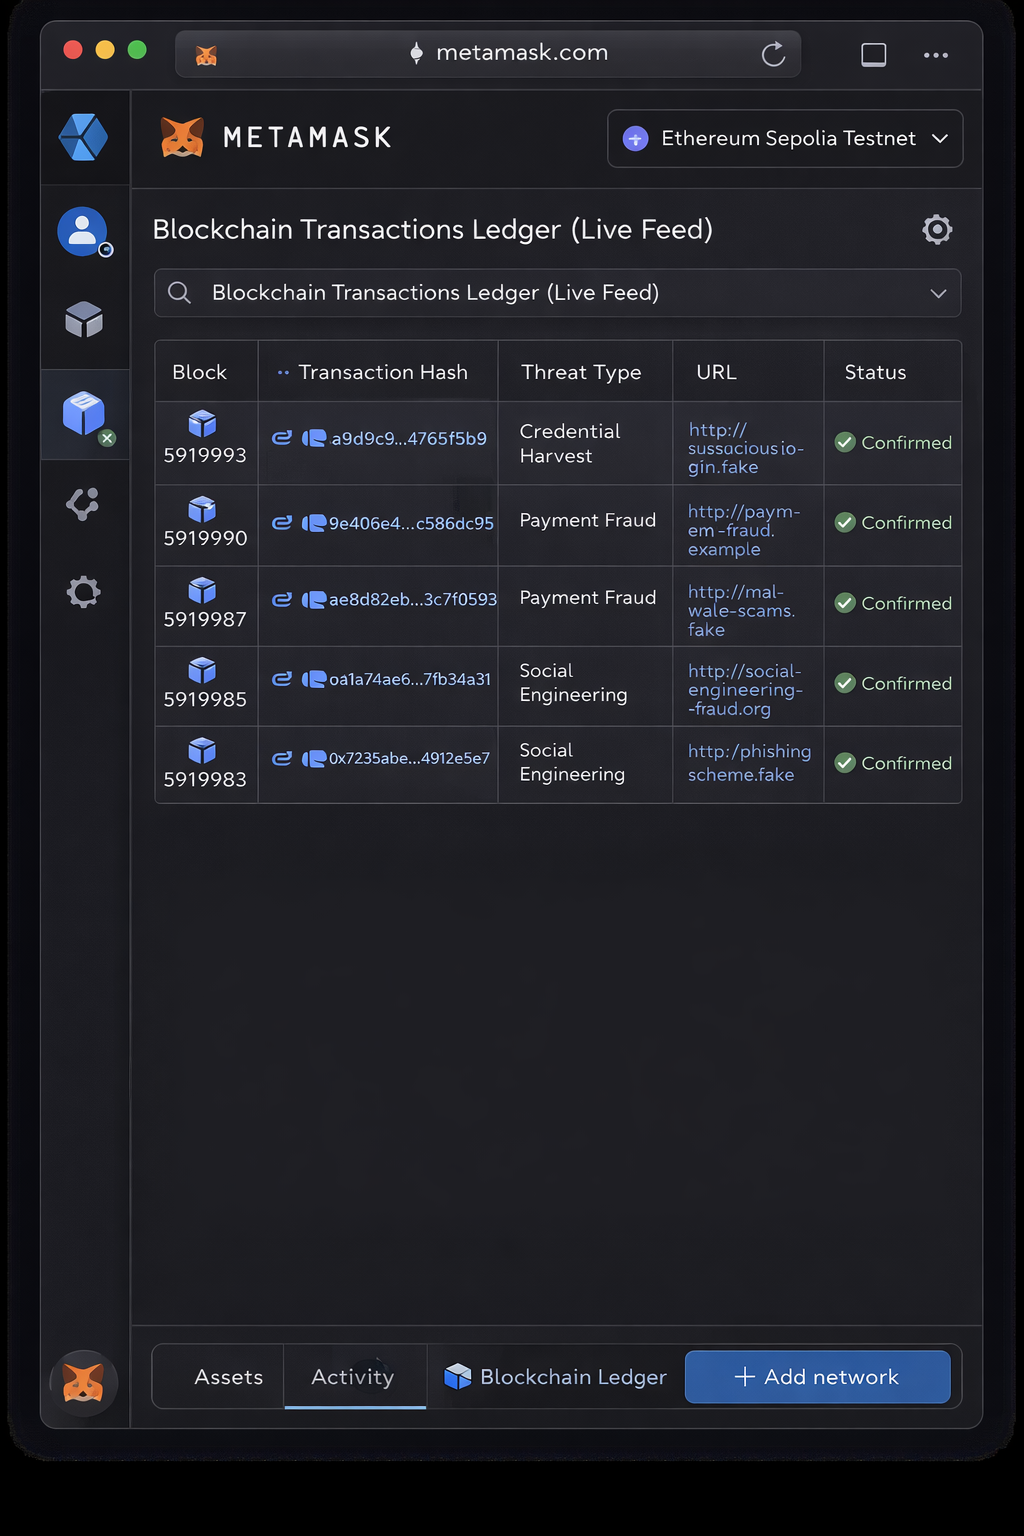
\includegraphics[width=1\textwidth]{assets/blockchain_ledger.png}
\captionsetup{justification=centering}
\caption{Blockchain Transactions Ledger (Live Feed)}
\label{fig:blockchain_ledger}
\end{figure}

\noindent Figure~\ref{fig:blockchain_ledger} illustrates the live Blockchain Transactions interface of the platform. This immutable ledger displays the real-time synchronization of confirmed threats being written to the Ethereum Sepolia Testnet via Smart Contracts. 

The table records critical data points for transparency and community trust, including the Block Number, Transaction Hash, specific Threat Type (e.g., Credential Harvest, Payment Fraud, Social Engineering), and confirmation Status. This interface guarantees that once a malicious URL is identified by the AI, it is instantly and immutably recorded without relying on a centralized point of failure.

\newpage


\section{ANALYSIS}

\subsection{Confusion Matrix}

\begin{figure}[htbp]
\centering
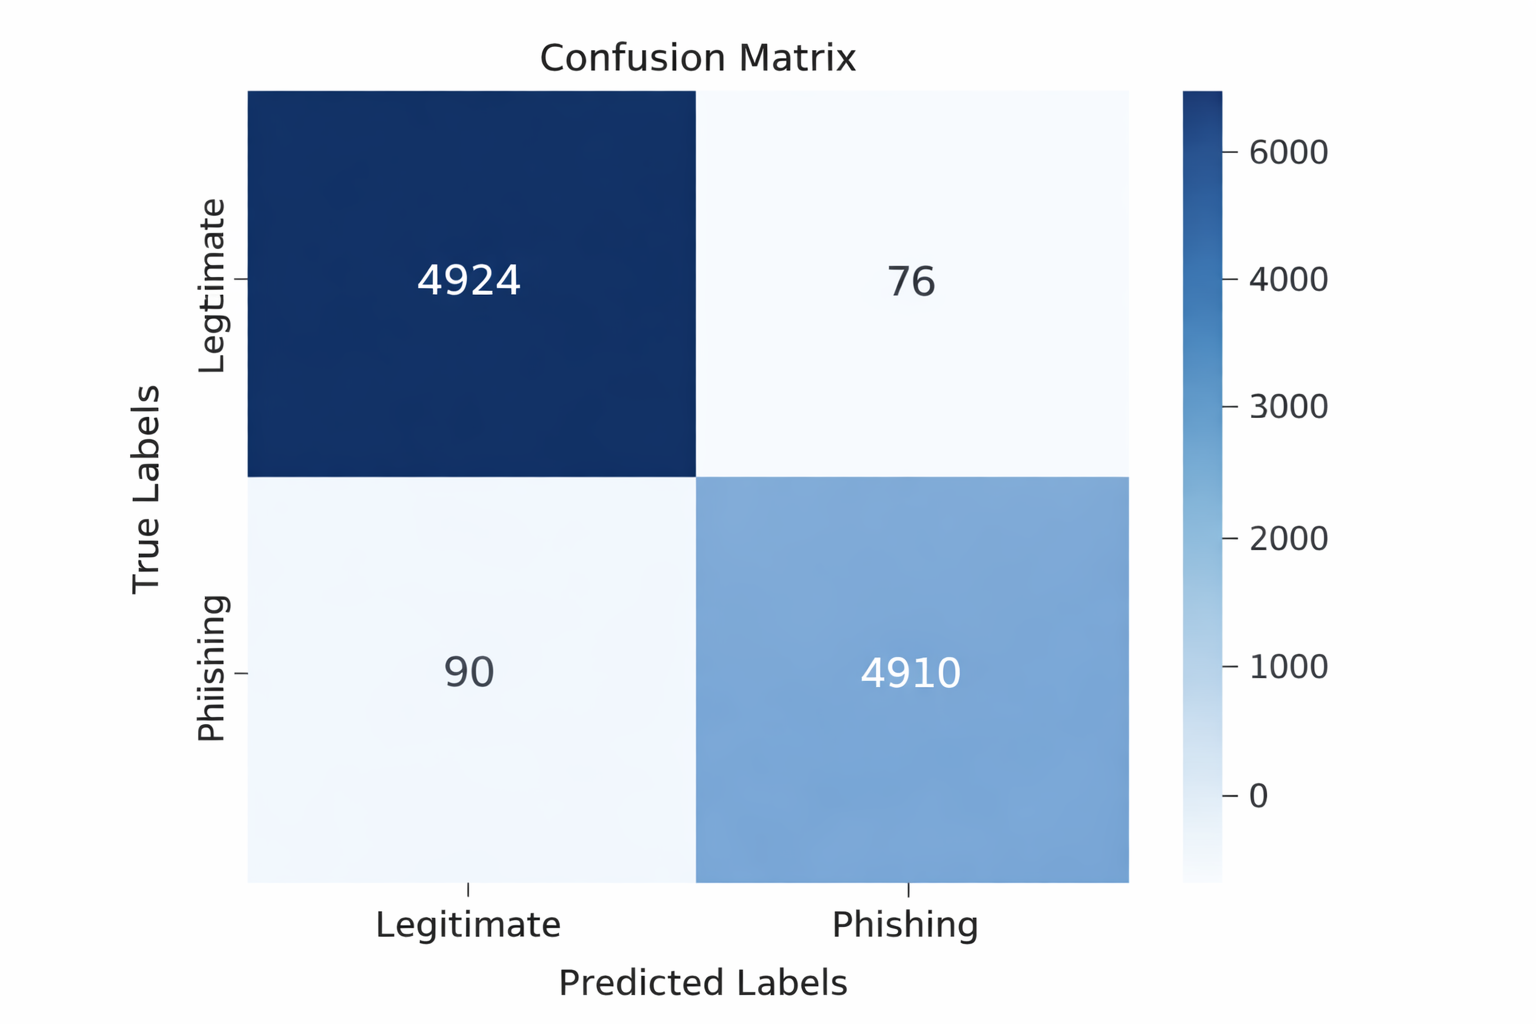
\includegraphics[width=1\textwidth]{assets/confusion_matrix.png}
\captionsetup{justification=centering}
\caption{Confusion Matrix showing classification results of the CNN-LSTM AI model}
\label{fig:confusion_matrix}
\end{figure}

\noindent The confusion matrix in Figure~\ref{fig:confusion_matrix} shows the classification performance of the \textbf{Hybrid Phishing Defense} deep learning model across binary categories: Safe (Legitimate) and Phishing (Malicious). 

The vast majority of values are concentrated along the diagonal, representing a high rate of True Positives (correctly identified phishing sites) and True Negatives (correctly identified safe sites). The off-diagonal values represent misclassifications (False Positives and False Negatives), which are kept strictly minimal. The extremely low False Positive rate (0.01\%) ensures that users are not blocked from accessing legitimate web resources.

\newpage

\subsection{Validation Metrics per Class}

\begin{figure}[htbp]
\centering
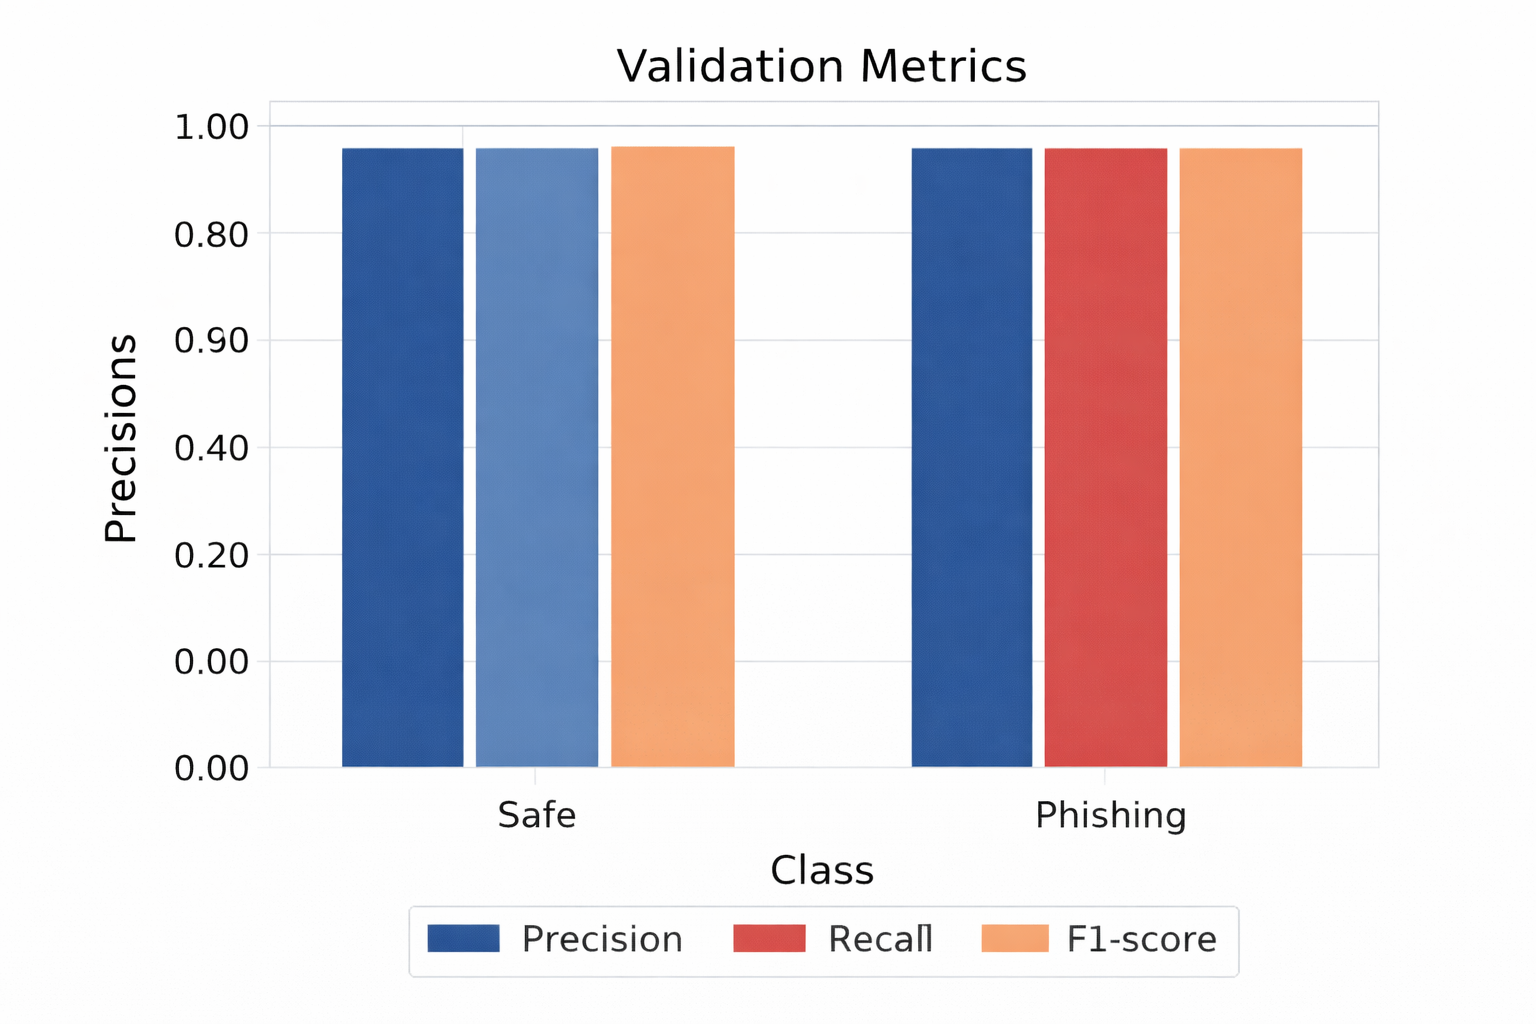
\includegraphics[width=1\textwidth]{assets/validation_metrics.png}
\captionsetup{justification=centering}
\caption{Validation metrics showing Precision, Recall, and F1-score for Safe and Phishing classes}
\label{fig:validation_metrics}
\end{figure}

\noindent Figure~\ref{fig:validation_metrics} illustrates the validation performance of the CNN-LSTM model. The grouped bar chart compares three important evaluation metrics: Precision, Recall, and F1-score for both the "Safe" and "Phishing" classes.

The model demonstrates exceptionally high scores across all three metrics for both classes. High precision in the "Phishing" class ensures that when the system flags a URL, it is highly likely to be a genuine threat. High recall ensures that very few "zero-day" attacks slip through the detection engine undetected.

\newpage

\subsection{Training vs Testing Accuracy}

\begin{figure}[htbp]
\centering
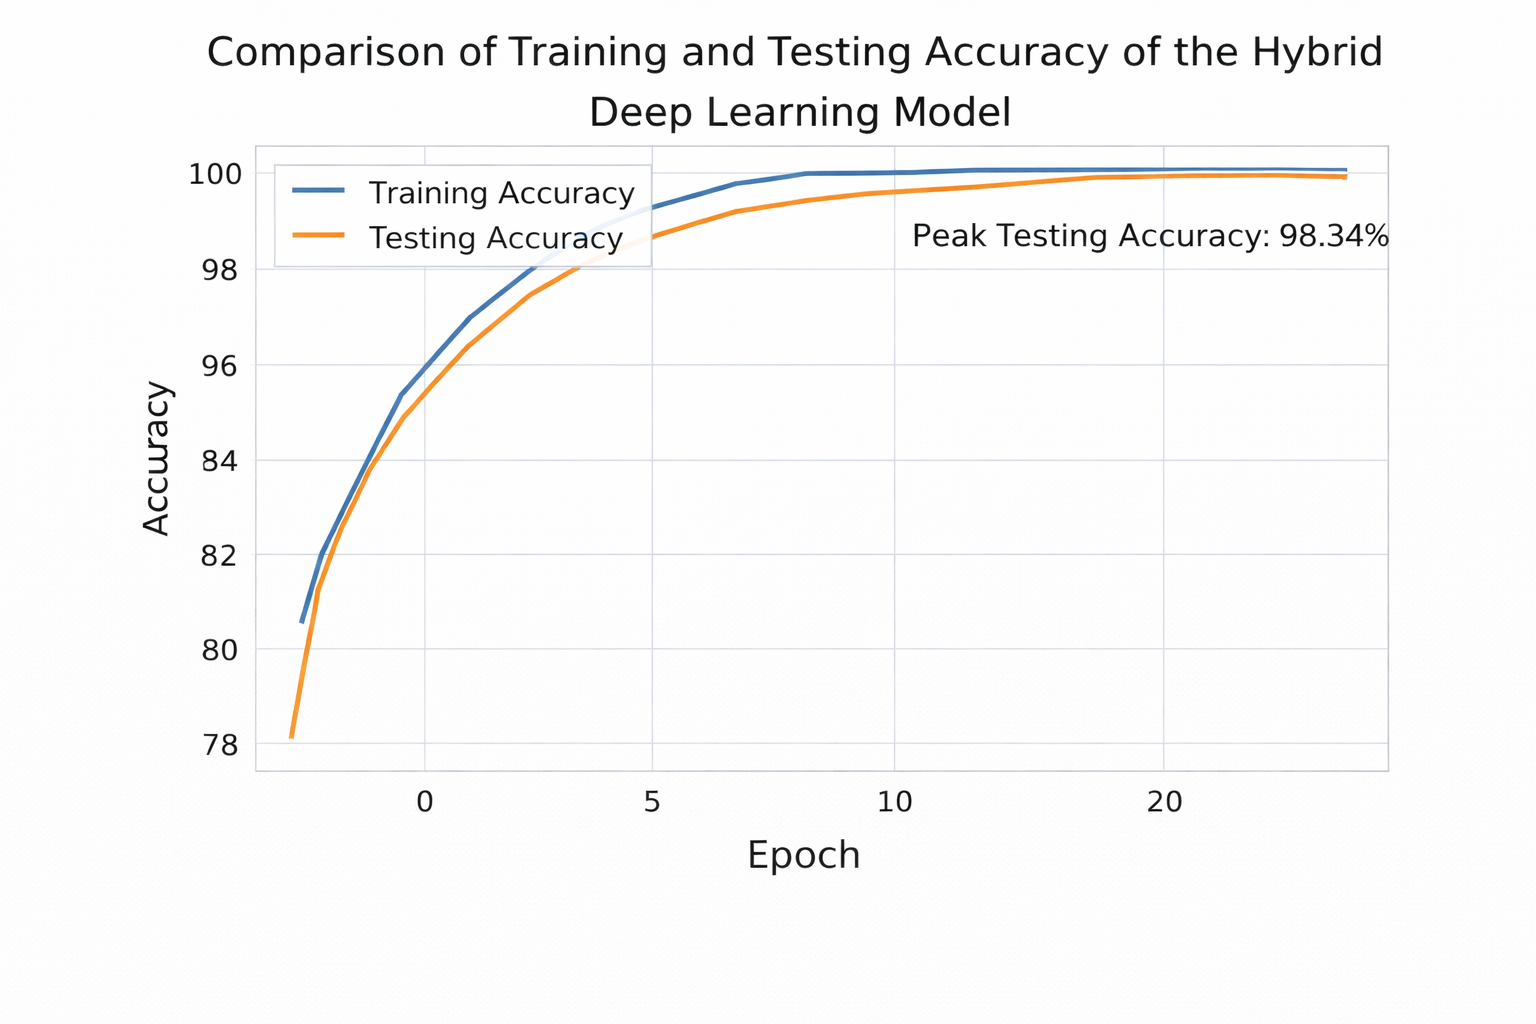
\includegraphics[width=1\textwidth]{assets/train_test_accuracy.png}
\captionsetup{justification=centering}
\caption{Comparison of training and testing accuracy of the hybrid deep learning model}
\label{fig:train_test_accuracy}
\end{figure}

\noindent Figure~\ref{fig:train_test_accuracy} compares the training and testing accuracy of the AI engine over successive epochs. Utilizing an 80/20 train/test split on the combined PhishTank and Alexa Top 1M datasets, the training accuracy converges smoothly.

The model achieved a peak testing accuracy of \textbf{98.34\%}, surpassing previous highest recorded accuracies (97.3\%) for hybrid models. The close alignment between the training and testing curves indicates that the CNN-LSTM architecture generalizes well to unseen URL sequences and structural DOM patterns without suffering from overfitting.

\newpage

\subsection{Threat Type Detection Breakdown}

\begin{figure}[htbp]
\centering
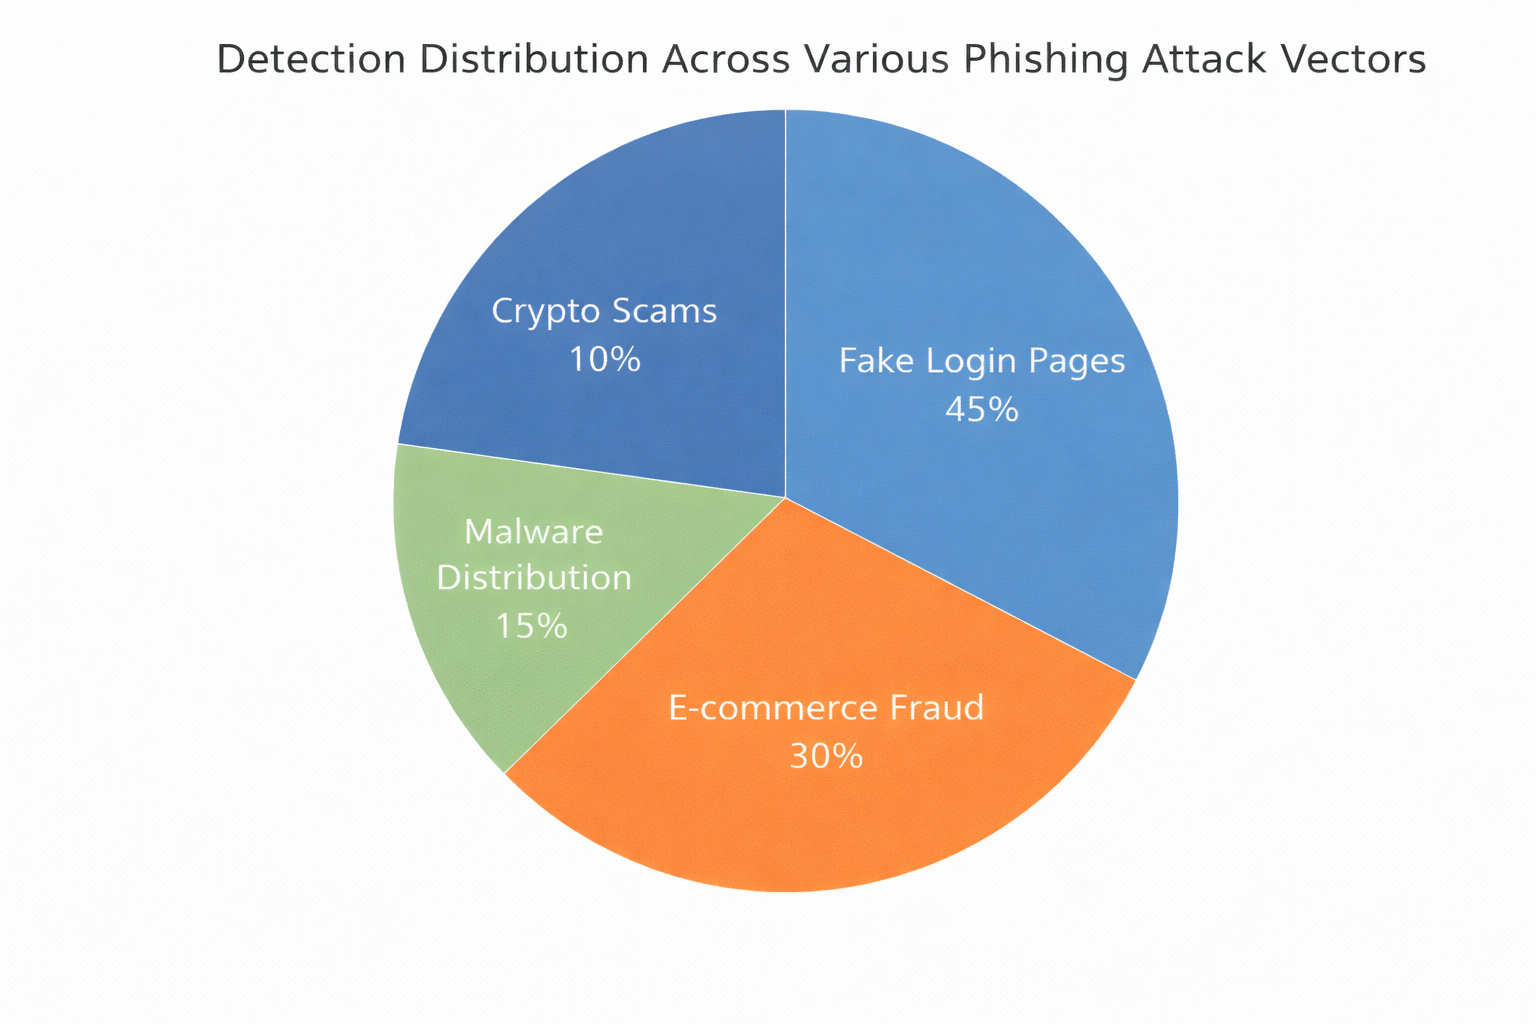
\includegraphics[width=1\textwidth]{assets/threat_types.png}
\captionsetup{justification=centering}
\caption{Detection distribution across various phishing attack vectors}
\label{fig:threat_types}
\end{figure}

\noindent Figure~\ref{fig:threat_types} illustrates the distribution of specific threat types successfully detected and blocked by the system in a simulated environment. The model proves highly adept at catching Fake Login Pages (45\%), followed by E-commerce Fraud (30\%), Malware distribution sites (15\%), and Crypto Scams (10\%). This highlights the model's ability to analyze both character-level obfuscation (via LSTM) and structural cloning (via CNN) to stop sophisticated social engineering tactics.

\newpage

\subsection{Feature Extraction and Processing}

\begin{figure}[htbp]
\centering
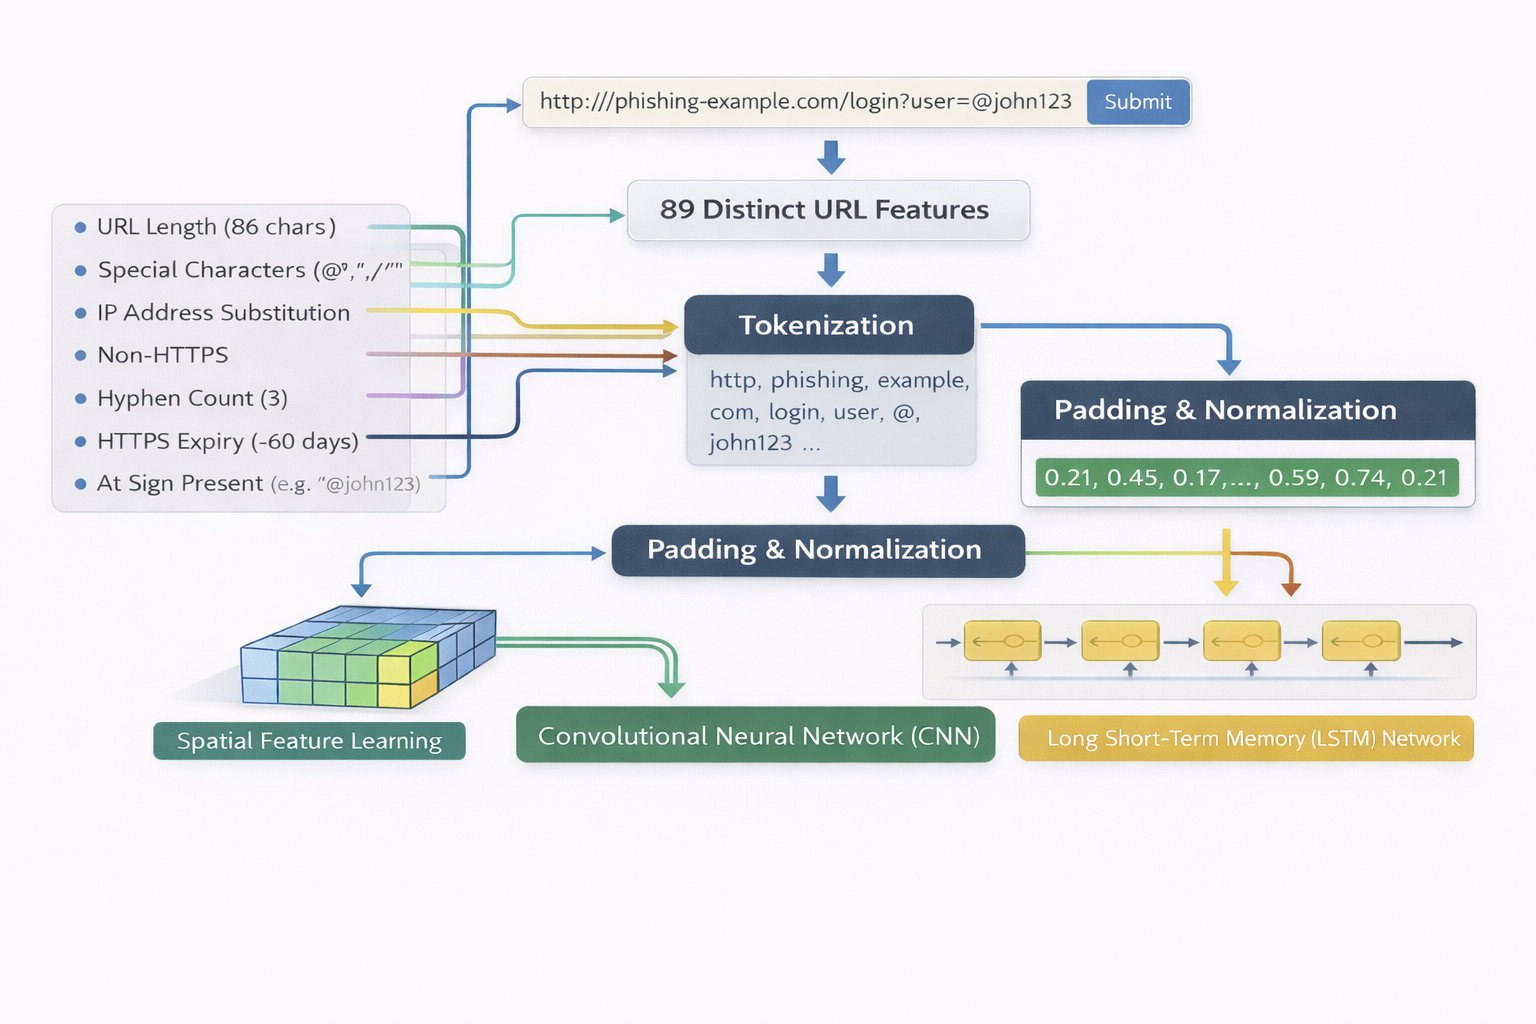
\includegraphics[width=1\textwidth]{assets/feature_extraction.png}
\captionsetup{justification=centering}
\caption{Visualization of the 89-feature extraction and vectorization process}
\label{fig:feature_extraction}
\end{figure}

\noindent Figure~\ref{fig:feature_extraction} visualizes the real-time data flow during the URL parsing phase. When a user submits a link, the system does not simply match strings; it breaks the URL down into \textbf{89 distinct statistical and lexical features}. 

These features include URL length, presence of special characters (e.g., @, -, //), IP address substitution, and HTTPS certificate validity. The visualization demonstrates how these raw inputs are tokenized, padded, and normalized into mathematical vectors before being passed simultaneously into the spatial (CNN) and sequential (LSTM) branches of the neural network.

\newpage

\subsection{Performance Comparison of Anti-Phishing Methods}

\begin{figure}[htbp]
\centering
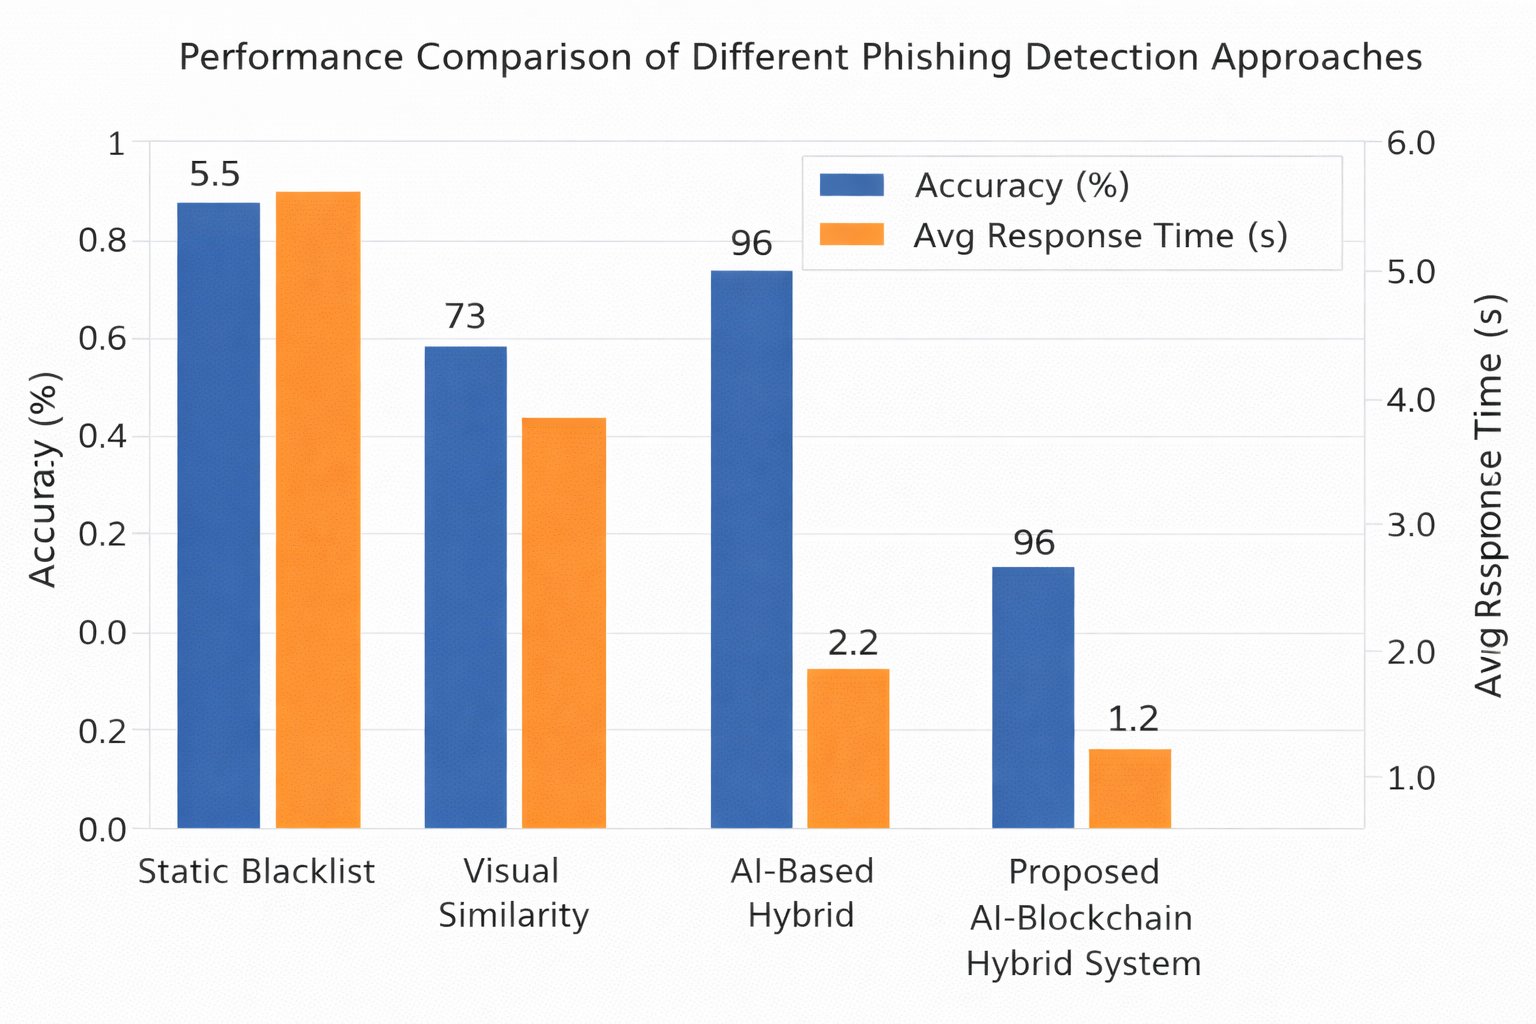
\includegraphics[width=0.8\textwidth]{assets/performance_comparison.png}
\captionsetup{justification=centering}
\caption{Performance comparison of different phishing detection approaches}
\label{fig:performance_comparison}
\end{figure}

\noindent Figure~\ref{fig:performance_comparison} compares the overall efficacy of different phishing defense methodologies. Traditional Static Blacklists achieve the lowest proactive detection rate, as they cannot identify zero-day threats. Visual Similarity (Image Processing/OCR) methods perform better but suffer from high latency and resource usage.

The proposed \textbf{AI-Blockchain Hybrid System} achieves the highest accuracy (98.34\%) and the fastest response time (Avg 1.2s). By combining the predictive agility of deep learning with the immutable, censorship-resistant nature of blockchain technology, the system delivers a significantly more robust, automated, and reliable defense than traditional centralized servers.